%---------------------------------------------------------------
\chapter{\babTiga}
%---------------------------------------------------------------

%-----------------------------------------------------------------------------%
\section{Sistem Arsitektur}
%-----------------------------------------------------------------------------%

\begin{figure}
	\centering
	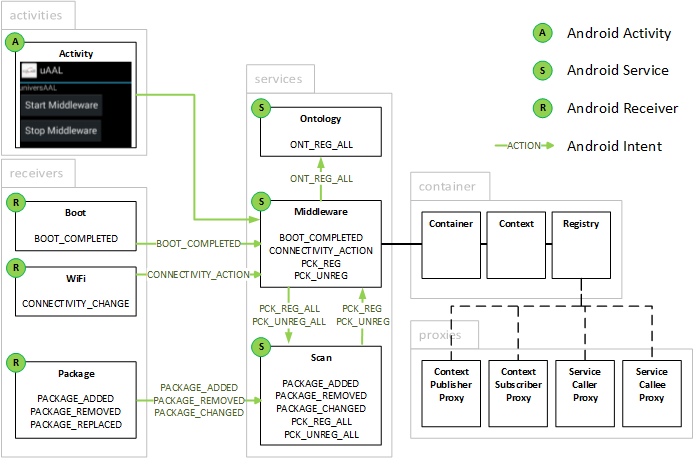
\includegraphics[width=0.9\textwidth]
	{pics/low_level.png}
	\caption{Low Level Design}
	\label{fig:31}
\end{figure}


\subsection{Gambaran Umum Sistem}
\blindtext \\

\subsection{Target Pengguna Aplikasi}
\blindtext \\

\subsection{Spesifikasi Target Perangkat}
\blindtext \\

\subsection{Diagram Alir Aplikasi}
\blindtext \\

%-----------------------------------------------------------------------------%
\section{Kebutuhan Pengembangan Sistem}
%-----------------------------------------------------------------------------%
\blindtext \\

\begin{table}[h]
	\centering
	\caption{List Software and Hardware}
	\label{tab:2}
	\begin{tabular}{ c c }
		\hline
		\textbf{Software} & \textbf{Hardware} \\ \hline \hline
		Microsoft Windows 10 & Processor minimal Intel Core i3	\\ 
		Android 7.1.2 (Nougat) & RAM 4 GB	\\ 
		Unity 3D 2018.2.4f1 & Hard disk 500 GB	\\ 
		Vuforia SDK 6-2-6 & Smartphone Android	\\ 
		Figma & Kamera minimal 5 MP	\\ \hline
	\end{tabular}
\end{table}


%-----------------------------------------------------------------------------%
\section{Perancangan Model Program}
%-----------------------------------------------------------------------------%
\blindtext \\

\subsection{Use Case Diagram}

\begin{figure}
	\centering
	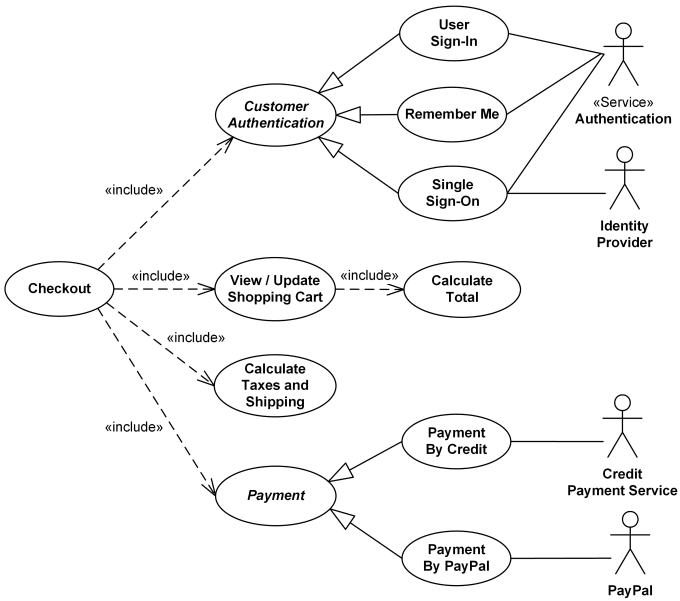
\includegraphics[width=0.9\textwidth]
	{pics/use-case-example.png}
	\caption{Online shopping UML use case diagram example}
	\label{fig:32}
\end{figure}

\subsection{Use Case Skenario}

%-----------------------------------------------------------------------------%
\section{Perancangan Aplikasi}
%-----------------------------------------------------------------------------%
\blindtext \\


\subsection{Perancangan Antar Muka}

\begin{figure}
	\centering
	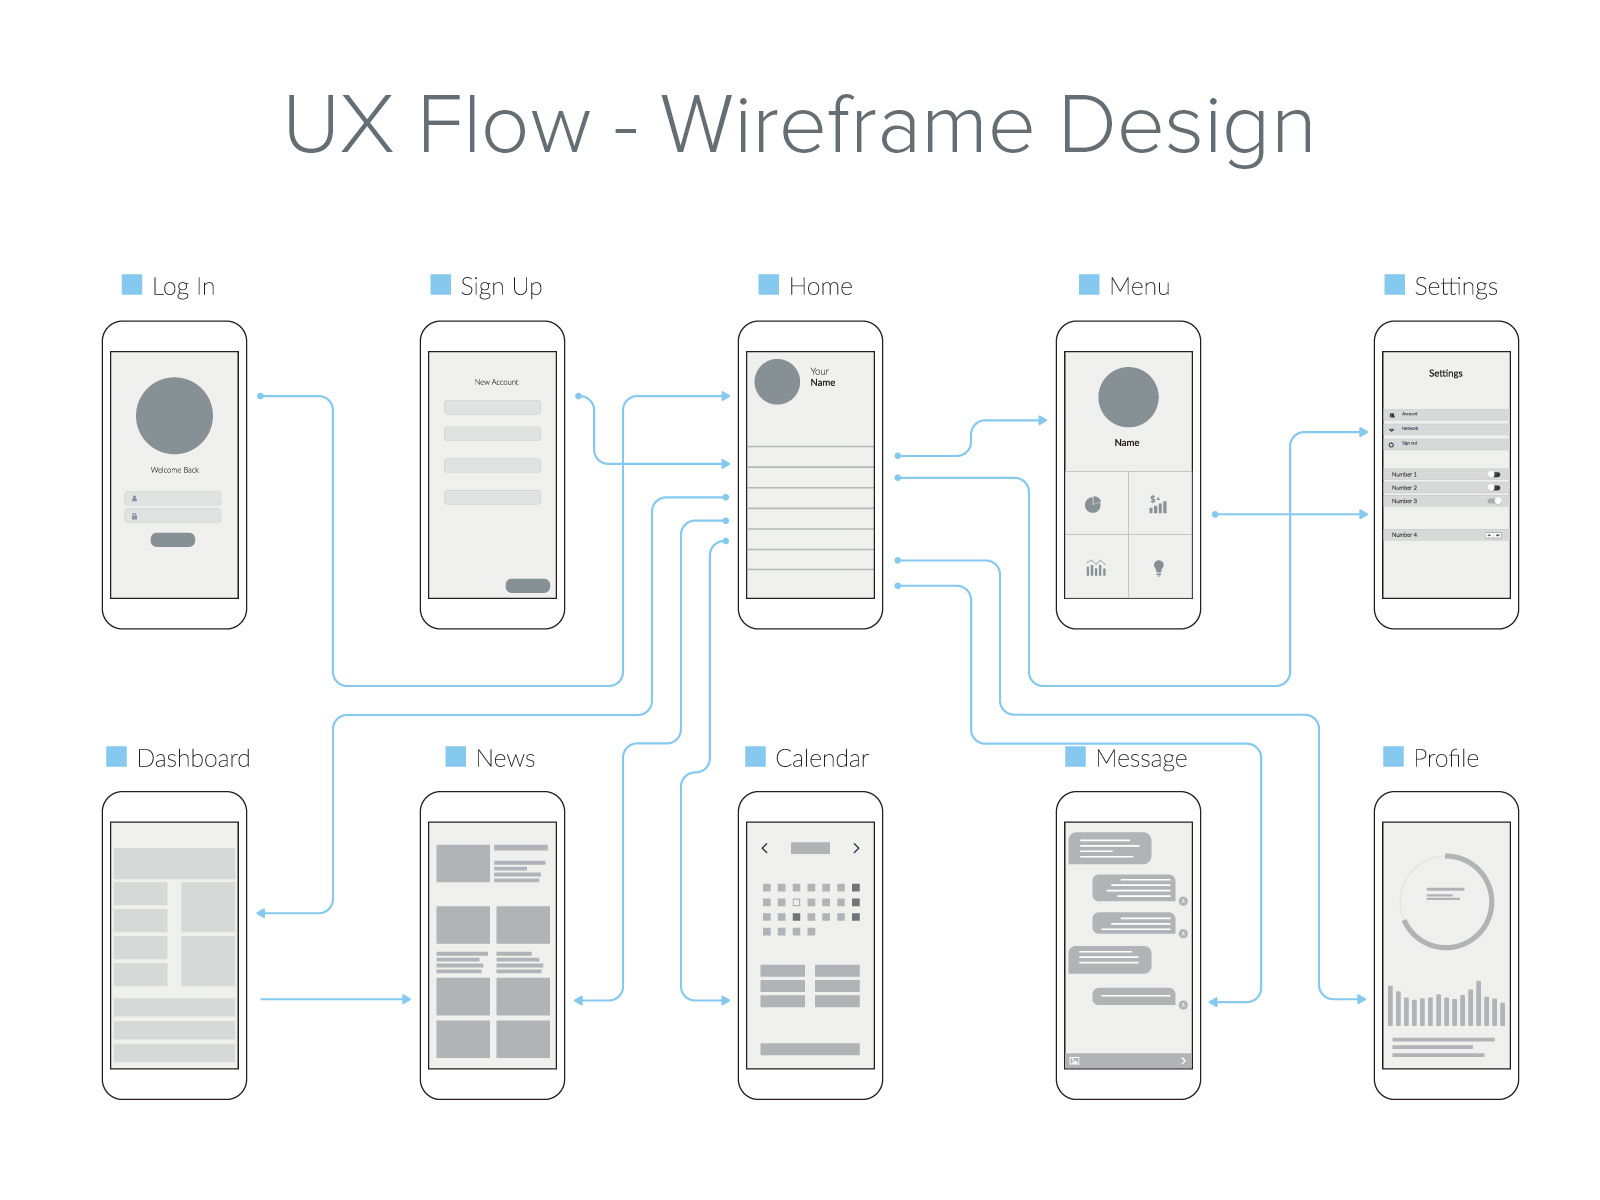
\includegraphics[width=0.9\textwidth]
	{pics/wireframe-design.jpg}
	\caption{Wireframe Design for Z-Apps}
	\label{fig:33}
\end{figure}

\blindtext \\

\subsection{Perancangan Level Tinggi}

\begin{figure}
	\centering
	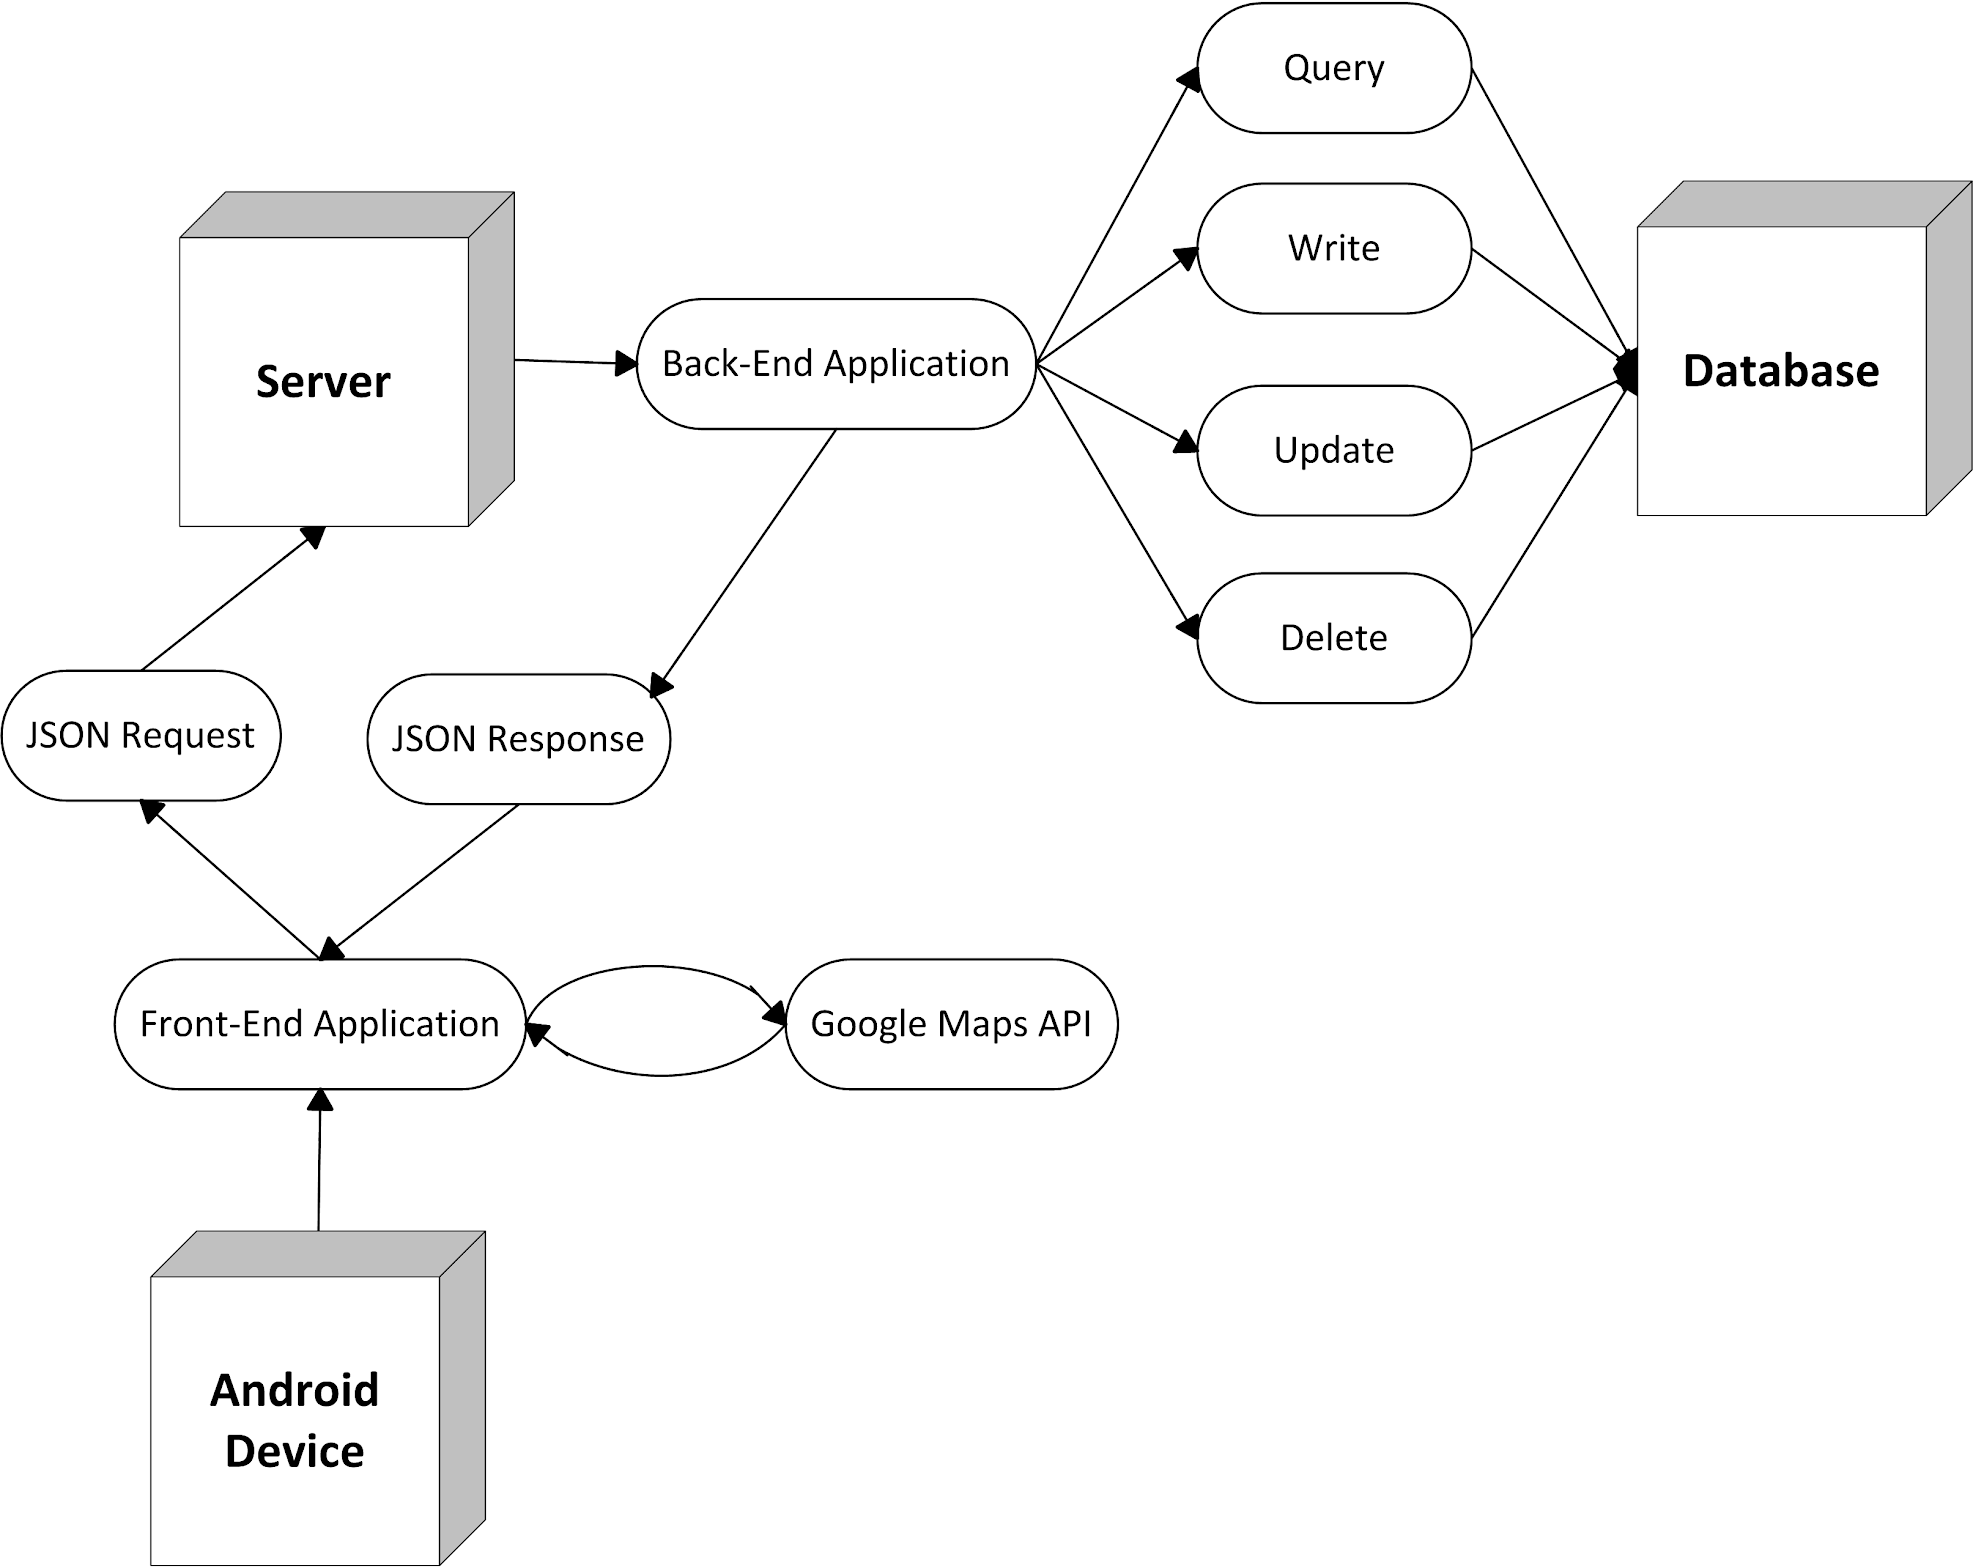
\includegraphics[width=0.9\textwidth]
	{pics/high_level.png}
	\caption{High Level Design}
	\label{fig:34}
\end{figure}

\blindtext \\
